% !TeX spellcheck = en_US
%\documentclass[11pt,a4paper]{article}
\documentclass[11pt
  , a4paper
  , article
  , oneside
%  , twoside
%  , draft
]{memoir}

\usepackage{control}
\usepackage[numbers]{natbib}

\newcommand{\newappendix}{%
  \refstepcounter{chapter}\chapter*{Appendix \thechapter}%
  \addcontentsline{toc}{chapter}{Appendix \thechapter}%
}

\begin{document}
	
\newcommand{\technumber}{
  RAON Control-Document Series\\
  Revision : v1.0,   Release : February 5, 2016}
\title{\textbf{Configuration of the Step motor control system using LS PLC on the EPICS}}

\author{Hyungjoo Son \\

  Rare Isotope Science Project\\
  Institute for Basic Science, Daejeon, South Korea
}
\date{\today}

\renewcommand{\maketitlehooka}{\begin{flushright}\textsf{\technumber}\end{flushright}}
%\renewcommand{\maketitlehookb}{\centering\textsf{\subtitle}}
%\renewcommand{\maketitlehookc}{C}
%\renewcommand{\maketitlehookd}{D}

\maketitle

\begin{abstract}\
  중이온 가속기에서 모든 제어환경은 EPICS에 통합될 예정이다. EPICS 환경에 로컬 제어시스템을 통합시키기 위해서는 로컬 제어시스템에서 각 디바이스들의 제어에 사용되는 PLC(Programmable Logic Controller)의 데이터들을 EPICS 환경으로 불러오는 과정이 필요하며, 이를 위해 EPICS IOC(Input Output Controller)를 구성하여 PV(Process Value)로 PLC의 데이터 값들을 관리하는 시스템을 구현해야 한다. 
  본 문서에서는 현재 제어실에 구성한 Step Motor testbed의 구동 시스템으로 사용된 LS PLC의 설정 방법에 대해서 간단히 기술하고, 이를 EPICS 환경에 통합하는 방법에 대해 설명할 것이다. 
\end{abstract}

\chapter{Step Motor control System의 구성}\
Step Motor Control System은 2개의 유한축과 1개의 무한장축으로 구성되어 있다. 2개의 유한축은 서로 연동되어 원호보간 운전 및 독립운전을 수행할 수 있으며, 1개의 무한장축은 리밋 센서와 상관없이 계속 회전할 수 있게 구성하였다. 모터들은 LS PLC에 의해서 구동되며 Local User Interface (UI) 로써 M2I사에서 생산되는 Touch panel을 사용하여 제어 시스템을 구성하였다. 이를 EPICS 환경에 통합시키기 위해서 EPICS에서 제공하는 Modbus 모듈을 이용하여 EPICS IOC를 구성하였으며, Local UI의 정보를 EPICS 환경에서 모니터링하기 위하여 Control System Studio (CSS)를 사용하여 모니터링 시스템을 구성하고 있다.    

\begin{figure}[h]
	\centering
	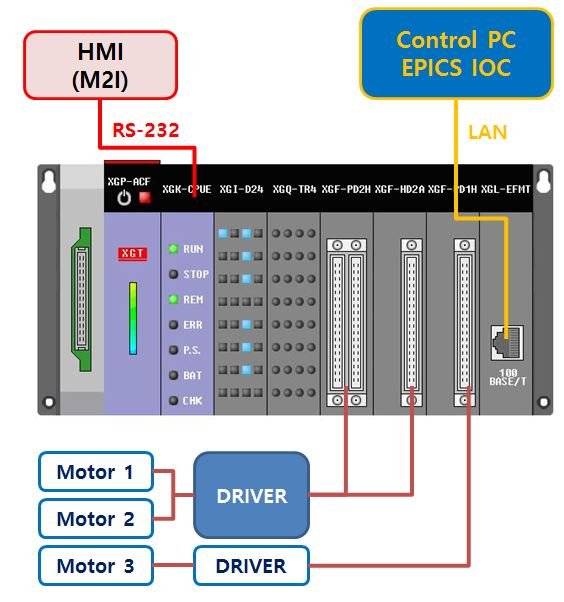
\includegraphics[width=0.8 \textwidth]{./picture/diagram.JPG}
	\caption{
		Step Motor Testbed configuration
	}
	\label{fig:}
\end{figure}


\section{장치 구성}\
다음은 Step Motor Control System의 구성요소이다. 현재 2개의 유한축에 설치된 모터들은 PLC부에 설치된 축카드에서 구동 신호를 주고 그 신호를 각각 모터 엔코더에서 받아서 모터를 구동하고, 움직인 정보를 고속 카운터에서 읽는 방식이다. 나머지 1개의 무한장축은 구동방식은 같으나 고속카운터 모듈은 설치되어 있지 않다. 

\begin{itemize}
\item Step Motor			: A15K-S545W (Autonics)
\item Motor encoder		    : E50S8 (Autonics)
\item Touch panel			: M2I TOP 8inch
\item PLC				    : LS PLC
\begin{itemize}
\item Power					: XGP-ACF2
\item CPU			        : XGI-CPUE
\item Digital input         : XGI-D24A
\item Digital Output	    : XGQ-TR4A
\item 2 Axis card		    : XGF-PD2H
\item 2 Axis counter		: XGF-HD2A
\item 1 Axis card		    : XGF-PD1H
\item modbusTCP card		: XGL-EFMT
\end{itemize}
\end{itemize}

\begin{figure}[h]
	\centering
	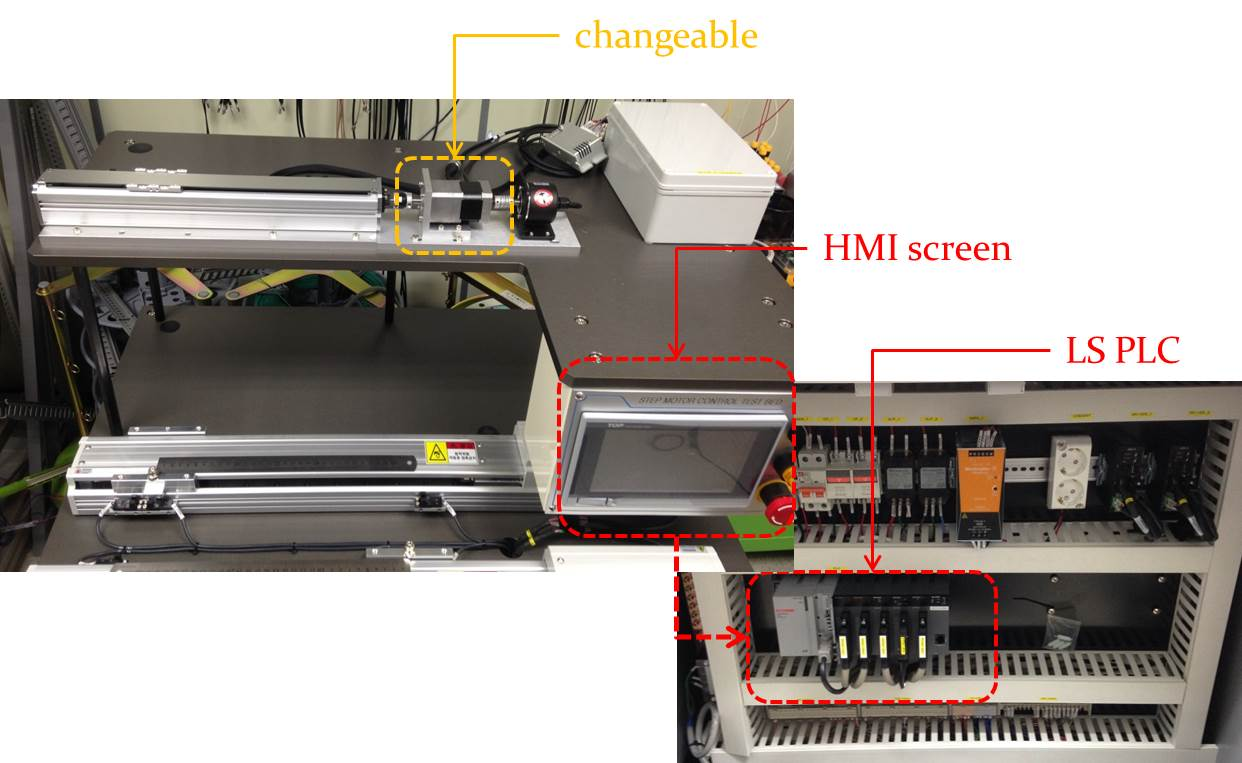
\includegraphics[width=0.8 \textwidth]{./picture/TESTBED_1.jpg}
	\caption{
		Step Motor testbed
	}
	\label{fig:}
\end{figure}

PLC CPU는 LS 에서 제조되는 상급 PLC인 CPUE 모델이 사용되었으며, Digital Input/Output 모듈은 24채널로 구성되었다. Step Motor의 설정 및 구동을 위한 축카드로는 유한축 2개를 구동할 수 있는 XGF-PD2H와 모터의 구동정보를 읽을 수 있는 XGF-HD2A가 설치되었으며, 무한장축 1개를 구동하기 위한 축카드 XGF-PD1H와 EPICS IOC와의 Modbus 통신을 위한 XGL-EFMT 모듈이 설치되었다. \\

Figure 2는 현재 구성된 Motor testbed의 모습이다. 유한축의 모터 2개는 고정되어 있으며, 무한장축의 모터는 모터의 종류에 따라 교체가 쉽도록 설치되어 있다. 모터의 제어와 모니터링을 위한 UI와 LS PLC는 RS-232로 연결되어 있다.

\newpage

\chapter{LS PLC Progarmming}\
 LS PLC의 CPUE 모델은 스크립트 형태로 프로그래밍 하는 ST(Statement), 입출력 및 명령어를 순차적으로 입력하는 LD(Ladder) 언어를 사용할 수 있다. FB(Function Block)의 언어를 사용하고 싶다면 LS 산전의 PLC 매뉴얼을 참조하여 해당 기능의 CPU모델을 사용하면 된다. 본 Step Motor control system은 PLC 프로그래밍에서 가장 일반적인 LD방식의 언어로 구성되어 있다. 

\section{PLC 입출력 메모리 구성}\
 LS PLC의 메모리 체계는 크게 Bit 와 Word 형태로 나뉜다. AB PLC의 경우 Tag의 형태로 메모리를 관리하여 Tag의 생성 시 메모리의 형태를 지정해줘야 하지만 LS PLC의 경우는 bit와 word 형태로만 구분하여 할당하면 된다. 또한 메모리는 내부 메모리와 실제 PLC 모듈에 지정되어 있는 외부 메모리로 구분할 수 있다. 내부 메모리는 유저가 임의대로 사용할 수 있는 영역과 시스템 자체 내에 할당되어 임의대로 사용할 수 없는 영역으로 나뉜다. bit 형태의 내부 메모리 M, P 등이 임의대로 사용할 수 있는 메모리에 해당하고, 타이머 메모리인 T의 형태와 점멸 비트 지정 메모리인 F 형태의 메모리 등이 임의대로 사용할 수 없는 영역에 해당한다. 외부 메모리는 PLC 모듈이 CPU에 연결될 때 자동으로 할당되는 메모리이다. 예를 들어, 16채널 Digital Input 카드가 CPU에 연결되어 있다면 16개의 bit는 Digital Input 카드가 사용할 수 있는 메모리로 할당되는 것이다. 이 외부 메모리의 경우 고정 할당식과 가변 할당식으로 또 나눌 수 있는데 이는 CPU타입에 따라 달라진다. CPU 모듈이 고정 할당식일 경우, 입출력 모듈의 접점수와는 상관없이 고정된 수의 메모리 영역이 할당된다. 만약 고정식 할당 CPU 바로 옆 슬롯에 Digital Input 16채널이 연결되어 있다면 P00000 번지 주소부터 P0000F 까지 할당되는 것은 가변식이고 채널수와 상관없이 CPU에서 지정된 메모리 영역만큼 할당되면 고정식이다.\\
 
 LS PLC의 메모리 형태의 상세 사항은 LS산전 홈페이지에서 다운 받을 수 있다.\
 Figure 3은 본 시스템에 설치된 PLC 모듈에 대한 메모리 상태이다.\

\begin{figure}[h]
	\centering
	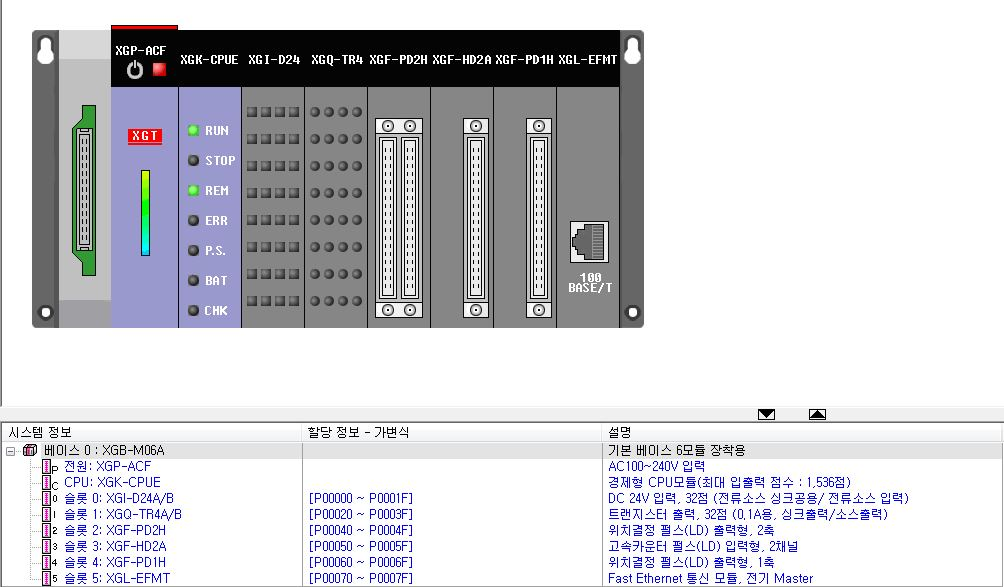
\includegraphics[width=1 \textwidth]{./picture/memory_assign.JPG}
	\caption{
		가변식 메모리 할당
	}
	\label{fig:}
\end{figure}

\begin{itemize}
\item Slot 0 : XGI-D24A/B, Input memory 32채널\\
Digigtal 형태의 Input 메모리는 CPU 모듈 바로 옆에 장착되어 있으며, 슬롯 0으로 할당된다. 32채널 모델이므로 P00000 부터 P0001F 까지 32개의 bit형 메모리가 Digital 입력모듈을 위해 할당된다. 메모리 정보에서 PLC CPU가 가변식인 것을 알 수 있다.   
\end{itemize}

\begin{itemize}
\item Slot 1 : XGQ-TR4A/B, Output memory 32채널\\
Digital 형태의 Ouptpu 메모리는 입력모듈 옆에 장착되어 있으며, 슬롯 1로 할당된다. 32채널 모델이므로 입력 모듈이 차지하고 있는 메모리 영역인 P0001F 이후 부터 32개의 bit형 메모리가 할당된다. P00020 부터 P0003F 까지 Digital 출력모듈을 위해 할당된다.  
\end{itemize}

\begin{itemize}
\item Slot 2 : XGF-PD2H, Axis card 2채널\\
Step Motor로 출력 펄스를 보내주는 모듈이다. 슬롯 2에 할당되어 있으며, P00040 부터 P0004F까지 16 개의 bit형 메모리가 할당된다.
\end{itemize}

\begin{itemize}
\item Slot 3 : XGF-HD2A, 고속카운터\\
Step Motor의 구동 정보를 펄스형태로 수신하는 모듈이다. 슬롯 3에 할당되어 있으며, P00050 부터 P0005F까지 16개의 bit형 메모리가 할당된다.
\end{itemize}

\begin{itemize}
\item Slot 4 : XGF-PD1H, Axis card 1채널\\
1채널 출력 펄스 모델로써 슬롯 4에 할당되어 있으며, P00060 부터 P0006F까지 15개의 bit형 메모리가 할당된다.
\end{itemize}

\begin{itemize}
\item Slot 5 : XGL-EFMT, Modbus communication card\\
EPICS Modbus 드라이브와 통신하기 위한 고속 이더넷 통신모듈이다. P00070부터 P0007F까지 16개의 Bit형 메모리가 할당된다.	
\end{itemize}


\newpage

 \section{PLC Programming software}\
LS PLC를 제어하기 위해서는 각 모듈의 기능에 맞는 소프트웨어를 사용해야 한다. 모든 소프트웨어는 무료이며, LS 산전 홈페이지에서 다운로드 할 수 있다. 본 문서에서는 제어 로직을 구성하기 위한 래더 프로그래밍 소프트웨어인 XG5000에 대해서 소개한다. 2014년에 배포된 XG5000은 이전에는 나뉘어져 있던 통신모듈 설정 소프트웨어의 기능이 통합되어 있다.  

XG5000은 설치된 모듈들의 등록 및 모듈 특성 설정,순차 제어 로직을 구성하는 프로그램으로서 입출력 및 다른 디바이스들과의 통신 로직을 구성할 수 있다. XG5000 역시 매뉴얼을 홈페이지에서 제공하나, 그 양이 방대하고 제어의 목적에 따라 사용하는 명령어가 다르므로 본 문서에서는 기본적인 입출력 구성과 Step Motor Testbed를 제어하기 위해 수행했던 통신설정 등을 위주로 XG5000의 기능을 설명한다. 기본 모듈 구성은 제조사에서 제공하는 매뉴얼을 참조하기 바란다. 
  
  \section{PLC connection and Module registration}
 PLC 제어환경을 구성하기 위해서는 먼저 제어용 PC와 PLC CPU와의 연결을 설정해야 한다. PC를 PLC CPU에 직접 연결할 때는 USB 케이블을 사용하여 로컬연결을 선택하여 PLC와 통신할 수 있으나, 원격 제어를 위해서는 LAN선을 연결할 수 있는 이더넷 모듈을 사용해야 한다. 본 시스템에서는 XGL-EFMT 모델을 원격제어용 모듈로 선정하였다.\
 
 PC와 PLC CPU 사이의 연결이 완료되면 장착된 PLC 모듈을 등록해줘야 해당 모듈을 사용할 수 있으며, 이 과정은 모든 메이커의 PLC에서 설정해야 하는 과정이다.
 
 \begin{figure}[h]
 	\centering
 	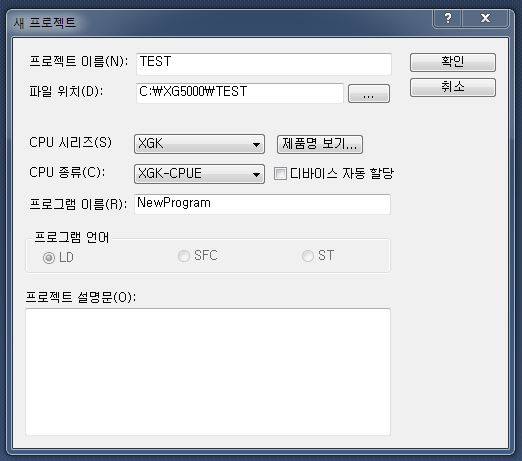
\includegraphics[width=0.6 \textwidth]{./picture/new_project.JPG}
 	\caption{
 		CPU module registration
 	}
 	\label{fig:}
 \end{figure}
 
 \newpage 
 
 XG5000을 실행한 후 PLC와 네트워크를 구성하는 방법과 각 모듈을 등록하는 방법을 아래에 설명한다. \\
 
 1) XG5000을 실행하면 상단 메뉴바 중 프로젝트 항목에서 새 프로젝트를 선택한다.\\
 
 2) 새 프로젝트 항목을 선택하면 Figure 4와 같은 화면이 팝업된다.\
 
    이 곳에 프로젝트 이름과 CPU 특성을 입력한다. 본 시스템은 XGK CPU 시리즈 중 CPUE 모델이 장착되어 있다.\
    
    CPUE 모듈은 Ladder 방식으로 프로그래밍이 되므로 프로그램 언어는 LD로 선택되어 진다.\\

 3) 확인 버튼을 눌러서 구성을 프로그램 초기 구성을 완료한다.\\
 
  \begin{figure}[h]
  	\centering
  	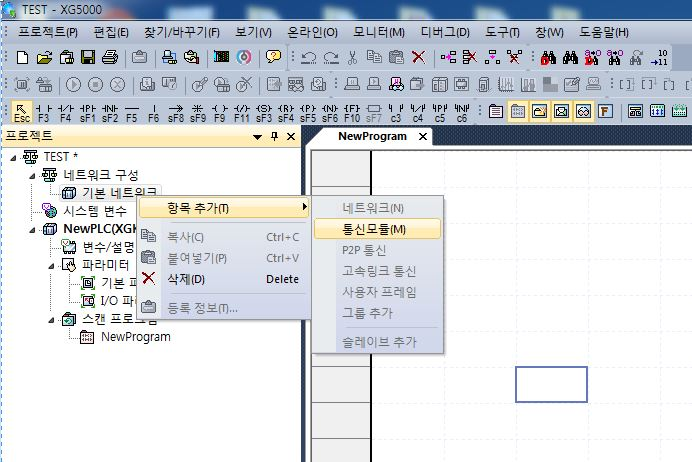
\includegraphics[width=0.85 \textwidth]{./picture/add_com_module.JPG}
  	\caption{
  		PLC communication module registration
  	}
  	\label{fig:}
  \end{figure}
 
  4) Figure 5와 같이 통신모듈을 추가시킨다. 모듈 선택창이 나오면 현재 시스템에 설치된 XGL-EFMT 모듈을 선택한다.\
  
    선택한 통신 모듈에 이름을 지정한다.\\
  
  5) 위의 과정이 끝나면 지정해준 네트워크 이름으로 기본네트워크가 구성된다.\\
  
  6) 구성된 네트워크 이름을 더블 클릭하여 통신모듈을 Figure 6과 같이 설정한다.\
     
     XGL-EFMT 모듈의 경우 LS산전의 전용통신인 XGT 서버와 모드버스 TCP/IP 서버로 사용될 수 있는데 드라이버 항목은 EPICS IOC의 Modbus 모듈을 사용할 것이므로 모드버스 TCP/IP를 선택한다.\\
     
  
  \begin{figure}[h]
  	\centering
  	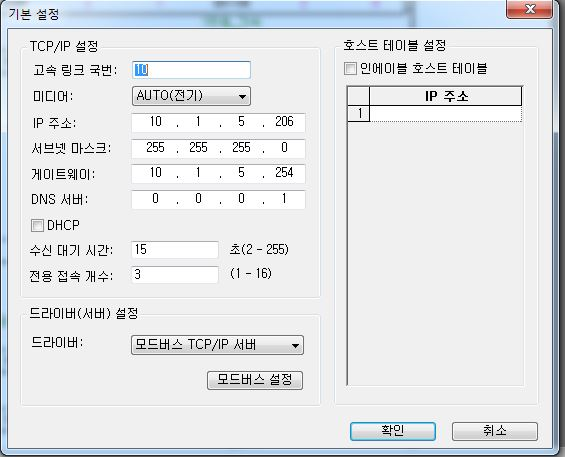
\includegraphics[width=0.55 \textwidth]{./picture/LS_modbus.JPG}
  	\caption{
  		Modbus Module setting
  	}
  	\label{fig:}
  \end{figure}
  
  \begin{figure}[h]
  	\centering
  	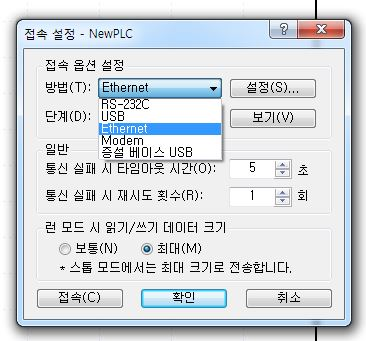
\includegraphics[width=0.55\textwidth]{./picture/ether-net.JPG}
  	\caption{
  		Connection setting
  	}
  	\label{fig:}
  \end{figure}
  
  
   \begin{figure}[h]
   	\centering
   	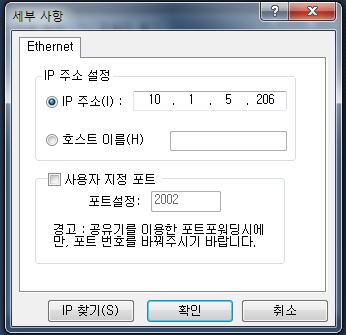
\includegraphics[width=0.55\textwidth]{./picture/LS_join_setting.JPG}
   	\caption{
   		Ip address setting 
   	}
   	\label{fig:}
  \end{figure}
  
   7) 통신 모듈에 대한 설정이 끝나면 상단 메뉴바의 온라인 항목을 선택한다.\
   
   접속설정 항목을 선택하여 PLC에 연결할 방법을 선택한다.\
   
   접속방법으로는 USB 모드 및 RS-232, Ether-net 등을 선택할 수 있는데, USB 모드는 PC와 PLC가 USB 케이블로 직접 연결되는 로컬 구성이고, 나머지 모드는 네트워크 환경에서 연결하는 구성이다. 리모트 모드를 선택한 후 Figure 8처럼 통신 모듈의 IP address를 입력한다. 확인 버튼을 눌러서 IP address 설정 메뉴를 나온다.\\
   
   8) 상단 메뉴바에서 온라인 항목의 연결 메뉴를 선택하여 PLC와 연결한다. \\
   
     \begin{figure}[h]
     	\centering
     	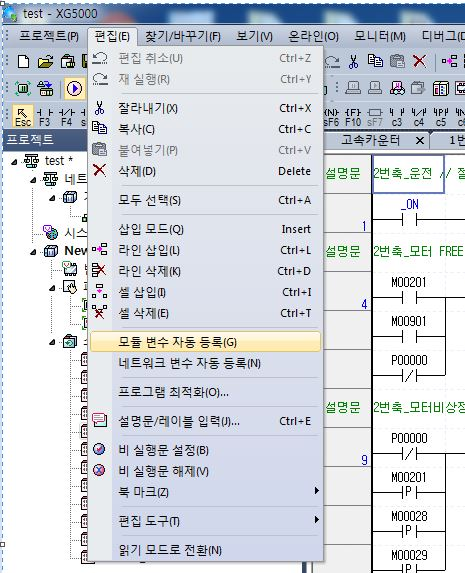
\includegraphics[width=0.7\textwidth]{./picture/module_var_regist.JPG}
     	\caption{
     		Module registration
     	}
     	\label{fig:}
     \end{figure}
  
   9) PLC와 연결이 완료되면 상단 메뉴에서 편집을 선택하여 현재 설치된 PLC module들을 등록한다.\
   
     Figure 9와 같이 모듈변수 자동등록을 선택하면 자동으로 PLC module을 등록함과 동시에 메모리도 자동으로 할당된다.\\ 
 
 
 \newpage
 
 위의 과정을 통해서 샷시에 설치된 모듈들을 모두 등록해야만 각 모듈에 해당하는 Tag 정보가 RSLogix5000에 등록되어 해당 모듈을 사용할 수 있다. \
 
 모듈 등록 과정이 끝나면 래더 프로그램을작성하기 위한 설정을 아래와 같이 진행한다.
 

\newpage
 
\chapter{EPICS IOC 와의 연동}
여기에서는 EPICS IOC와 LS PLC 데이터 통신에 대해서 알아본다. EPICS 환경을 구성하는 방법은 Script\_for\_epics(https://github.com/jeonghanlee/scripts\_for\_epics)를 참조하기 바라며, EPICS IOC와 LS PLC 간의 데이터 통신을 위한 드라이버는 modbus-2-7(http://cars9.uchicago.edu/software/epics/modbus.html)를 사용했다. \\

\section{RELEASE file 설정}
EPICS IOC 생성 후 ~/epics/R3.14.12.5/siteApps/your IOC/configure/RELEASE 파일을 다음과 같이 설정한다. 파일의 경로는 PC의 EPICS의 환경에 따라 다르다.\\

\begin{lstlisting}[style=termstyle]

TEMPLATE_TOP=$(EPICS_BASE)/templates/makeBaseApp/top

# If using the sequencer, point SNCSEQ at its top directory:
#SNCSEQ=$(EPICS_BASE)/../modules/soft/seq

ASYN=${EPICS_SYNAPPS}/asyn-4-26
MODBUS=${EPICS_SYNAPPS}/modbus-2-7

# EPICS_BASE usually appears last so other apps can override stuff:
EPICS_BASE=/home/sonhyungjoo/epics/R3.14.12.5/base

# Set RULES here if you want to take build rules from somewhere
# other than EPICS_BASE:
#RULES=/path/to/epics/support/module/rules/x-y


\end{lstlisting}

RELEASE 파일은 supprot module의 경로를 지정해주는 파일이다. 여기에서는 AB PLC와 EPICS IOC간의 통신을 위한 Modbus Driver(MODBUS=\${EPICS\_SYNAPPS}/modbus-2-7)가 저장되어 있는 경로를 지정해 준다.\

\section{Db Makefile 설정}

Db Makefile은 AB PLC의 Tag를 EPICS IOC의 PV와 일치시키기 위한 db파일을 등록하는 파일이다. Tag의 데이터 형태에 따라 db파일을 생성한 후 Db 디렉토리에 추가해 준다. 현재의 시스템에서의 경로는 '/epics/R3.14.12.5/siteApps/lsplcModbus/lsplcApp/Db/Makefile'이다.\
 
\begin{lstlisting}[style=termstyle]

TOP=../..
include $(TOP)/configure/CONFIG
#----------------------------------------
#  ADD MACRO DEFINITIONS AFTER THIS LINE

#----------------------------------------------------
#  Optimization of db files using dbst (DEFAULT: NO)
#DB_OPT = YES

#----------------------------------------------------
# Create and install (or just install) into <top>/db
# databases, templates, substitutions like this
DB += bi_word.template
DB += bo_word.template
DB += bi_bit.template
DB += bo_bit.template
DB += longin.template
DB += longout.template
DB += longinInt32.template
DB += longoutInt32.template
DB += mbbiDirect.template
DB += mbboDirect.template
DB += ai.template
DB += ai_average.template
DB += ao.template
DB += aiFloat64.template
DB += aoFloat64.template
DB += intarray_in.template
DB += intarray_out.template
DB += statistics.template
DB += asynRecord.template
DB += poll_delay.template


\end{lstlisting}

\section{src Makefile 설정}

src Makefile은 support module의 Library 및 dbd 파일의 정보를 등록하는 파일이다. 현재 시스템에서의 경로는 '/epics/R3.14.12.5/siteApps/lsplcModbus/lsplcApp/src/Makefile'이다.\

\begin{lstlisting}[style=termstyle]
TOP=../..

include $(TOP)/configure/CONFIG
#----------------------------------------
#  ADD MACRO DEFINITIONS AFTER THIS LINE
#=============================

#=============================
# Build the IOC application

PROD_IOC = lsplc
# lsplc.dbd will be created and installed
#DBD += $(MODBUS)/dbd/modbus.dbd
DBD += $(MODBUS)/dbd/modbusSupport.dbd
DBD += $(ASYN)/dbd/drvAsynIPPort.dbd
DBD += $(ASYN)/dbd/asyn.dbd
DBD += lsplc.dbd

# lsplc.dbd will be made up from these files:
lsplc_DBD += base.dbd
lsplc_DBD += $(TOP)/dbd/modbusSupport.dbd
lsplc_DBD += $(TOP)/dbd/drvAsynIPPort.dbd
lsplc_DBD += $(TOP)/dbd/asyn.dbd

# Include dbd files from all support applications:

# Add all the support libraries needed by this IOC
#lsplc_LIBS += xxx
lsplc_LIBS += asyn modbus

# lsplc_registerRecordDeviceDriver.cpp derives from lsplc.dbd
lsplc_SRCS += lsplc_registerRecordDeviceDriver.cpp

# Build the main IOC entry point on workstation OSs.
lsplc_SRCS_DEFAULT += lsplcMain.cpp
lsplc_SRCS_vxWorks += -nil-

# Add support from base/src/vxWorks if needed
#lsplc_OBJS_vxWorks += $(EPICS_BASE_BIN)/vxComLibrary

# Finally link to the EPICS Base libraries
lsplc_LIBS += $(EPICS_BASE_IOC_LIBS)

#===========================

include $(TOP)/configure/RULES


\end{lstlisting}


\section{Record file 작성}

Record file은 LS PLC에서 사용되고 있는 메모리 address를 EPICS IOC PV와 일치시키기 위해 작성하는 파일이다. EPICS record file을 작성하는 Reference를 EPICS 홈페이지에서 확인할 수 있다.\\

아래의 record file은 Digital Input/Output 값을 제어하기 위한 파일이다. 현재 시스템에서의 경로는 '/epics/R3.14.12.5/siteApps/lsplcModbus/lsplcApp/Db/bi\_bit.template'이다. \\

\begin{lstlisting}[style=termstyle]

# bi record template for register inputs
record(bi,"$(P)$(R)") {
field(DTYP,"asynUInt32Digital")
field(INP,"@asynMask($(PORT) $(OFFSET) 0x1)")
field(SCAN,"$(SCAN)")
field(ZNAM,"$(ZNAM)")
field(ONAM,"$(ONAM)")
field(ZSV,"$(ZSV)")
field(OSV,"$(OSV)")
}

\end{lstlisting}

Record file은 PLC 측의 Digital Input 모듈로 입력되는 신호를 EPICS IOC PV로 가져오기 위한 과정이다. 만약 설정해줘야 할 항목들이 많다면 별도의 template을 만들어서 관리할 수 있다. 예를 들어 위의 record file은 하나의 입력 bit를 설정해 주기 위해서 10줄에 해당하는 스크립트를 구성하였다. 10개의 입력 bit를 제어하려 한다면 그에 해당하는 스크립트도 길어지기 마련이다. 이를 해결하기 위해 별도의 template file을 만들어서 관리한다.\\

아래의 template file은 PLC에 할당된 bit 및 word를 EPICS IOC PV와 일치시키기 위한 file이다. 현재 시스템에서의 경로는 '/epics/R3.14.12.5/siteApps/lsplcModbus/iocBoot/ioclsplc/StepMTst\_pre.substitutions'이다. \\

\begin{lstlisting}[style=termstyle]

# These are the Digital Coil inputs with StepMTst
file "../../db/bi_bit.template" { pattern
{P,           R,         PORT,             OFFSET,   ZNAM,   ONAM,  ZSV,       OSV,    SCAN}
{STEP:,    CInB0,     Step_Motor_CIn_Bit,     0,     Low,    High,  NO_ALARM,  MAJOR,  "I/O Intr"}
{STEP:,    CInB1,     Step_Motor_CIn_Bit,     1,     Low,    High,  NO_ALARM,  MAJOR,  "I/O Intr"}
{STEP:,    CInB2,     Step_Motor_CIn_Bit,     2,     Low,    High,  NO_ALARM,  MAJOR,  "I/O Intr"}
{STEP:,    CInB3,     Step_Motor_CIn_Bit,     3,     Low,    High,  NO_ALARM,  MAJOR,  "I/O Intr"}
{STEP:,    CInB4,     Step_Motor_CIn_Bit,     4,     Low,    High,  NO_ALARM,  MAJOR,  "I/O Intr"}
{STEP:,    CInB5,     Step_Motor_CIn_Bit,     5,     Low,    High,  NO_ALARM,  MAJOR,  "I/O Intr"}
{STEP:,    CInB6,     Step_Motor_CIn_Bit,     6,     Low,    High,  NO_ALARM,  MAJOR,  "I/O Intr"}
{STEP:,    CInB7,     Step_Motor_CIn_Bit,     7,     Low,    High,  NO_ALARM,  MAJOR,  "I/O Intr"}
{STEP:,    CInB8,     Step_Motor_CIn_Bit,     8,     Low,    High,  NO_ALARM,  MAJOR,  "I/O Intr"}
{STEP:,    CInB9,     Step_Motor_CIn_Bit,     9,     Low,    High,  NO_ALARM,  MAJOR,  "I/O Intr"}
{STEP:,    CInB10,     Step_Motor_CIn_Bit,    10,     Low,    High,  NO_ALARM,  MAJOR,  "I/O Intr"}
{STEP:,    CInB11,     Step_Motor_CIn_Bit,    11,     Low,    High,  NO_ALARM,  MAJOR,  "I/O Intr"}
{STEP:,    CInB12,     Step_Motor_CIn_Bit,    12,     Low,    High,  NO_ALARM,  MAJOR,  "I/O Intr"}
{STEP:,    CInB13,     Step_Motor_CIn_Bit,    13,     Low,    High,  NO_ALARM,  MAJOR,  "I/O Intr"}
{STEP:,    CInB14,     Step_Motor_CIn_Bit,    14,     Low,    High,  NO_ALARM,  MAJOR,  "I/O Intr"}
{STEP:,    CInB15,     Step_Motor_CIn_Bit,    15,     Low,    High,  NO_ALARM,  MAJOR,  "I/O Intr"}
}

file "../../db/bo_bit.template" { pattern
{P,        R,              PORT,              OFFSET,   ZNAM,   ONAM}
{STEP:,    COutB0,     Step_Motor_COut,     0,        Low,    High}
{STEP:,    COutB1,     Step_Motor_COut,     1,        Low,    High}
{STEP:,    COutB2,     Step_Motor_COut,     2,        Low,    High}
{STEP:,    COutB3,     Step_Motor_COut,     3,        Low,    High}
{STEP:,    COutB4,     Step_Motor_COut,     4,        Low,    High}
{STEP:,    COutB5,     Step_Motor_COut,     5,        Low,    High}
{STEP:,    COutB6,     Step_Motor_COut,     6,        Low,    High}
{STEP:,    COutB7,     Step_Motor_COut,     7,        Low,    High}
{STEP:,    COutB8,     Step_Motor_COut,     8,        Low,    High}
{STEP:,    COutB9,     Step_Motor_COut,     9,        Low,    High}
{STEP:,    COutB10,     Step_Motor_COut,     10,        Low,    High}
{STEP:,    COutB11,     Step_Motor_COut,     11,        Low,    High}
{STEP:,    COutB12,     Step_Motor_COut,     12,        Low,    High}
{STEP:,    COutB13,     Step_Motor_COut,     13,        Low,    High}
{STEP:,    COutB14,     Step_Motor_COut,     14,        Low,    High}
{STEP:,    COutB15,     Step_Motor_COut,     15,        Low,    High}
}


\end{lstlisting}

위의 StepMTst\_pre.substitutions file은 Digital Input 16채널과 Digital Output 16채널의 PV를 설정한다. Integer 형태 및 Float 형태의 Analog 형태의 데이터 값도 위와 같이 구성할 수 있다.

\section{st.cmd file 작성}

st.cmd file은 EPICS IOC를 실행하는 파일이다. LS PLC의 IP address 및 데이터 교환 방식을 설정해 준다.  

\begin{lstlisting}[style=termstyle]
	
#!../../bin/linux-x86_64/lsplc

## You may have to change lsplc to something else
## everywhere it appears in this file

< envPaths

cd "${TOP}"

## Register all support components
dbLoadDatabase "dbd/lsplc.dbd"
lsplc_registerRecordDeviceDriver pdbbase

drvAsynIPPortConfigure("StepMTst","10.1.5.206:502",0,0,1)
modbusInterposeConfig("StepMTst",0,5000,0)

# The LSPLC - XGT - modbusTCP, Function code
# Read 32 bits, Discret Input.  Function code=2.

#drvModbusAsynConfigure("1", "2",3 ,4,"octal value", 6, 7 ,8,9)
#-> PLC PXXXXX -> Hexa value, octal value convert to Hexa, refer LS-PLC XGK-EFMT Memory Address
# Address = 1XXXX, Response Length = 2000 Coils(2000bits)
drvModbusAsynConfigure("Step_Motor_CIn_Bit",   "StepMTst", 0, 1,  0x0C0, 100,    0,  100, "Modicon")

# Write 1 bit.  Function code=5.
# Address = 0XXXX, Response Length = 1 Coil(1bits)

drvModbusAsynConfigure("Step_Motor_COut",  "StepMTst", 0, 5,  0x100,  100,    0,  1, "Modicon")


# drvModbusAsynConfigure("portName", "tcpPortName", slaveAddress, modbusFunction, modbusStartAddress, modbusLength, dataType,$
## drvModbusAsynConfigure("A0_Out_Word", "sim1", 0, 16, 100, 10, 7, 1, "Simulator")

# Write Analog Out (INT 32bit). Function code= 16.

drvModbusAsynConfigure("Step_Motor_AOut", "StepMTst",  0, 16, 300, 30,   5,  1, "Modicon")

# Write Analog Input (UNINT). Function code= 16.

drvModbusAsynConfigure("Step_Motor_AIn", "StepMTst", 0, 16, 350, 30,  5,  1, "Modicon")



# Write Analog Out (Float).

drvModbusAsynConfigure("Step_Motor_FOut", "StepMTst", 0, 16, 400, 30,   7,  1, "Modicon")

# Write Analog Input (Float).

drvModbusAsynConfigure("Step_Motor_FIn", "StepMTst", 0, 16, 450, 30,   7,  1, "Modicon")


	
\end{lstlisting}


\section{PLC 와 EPICS IOC 통신의 예}

위의 st.cmd file에서 Digital Output 설정을 예를 들어보면, drvModbusAsynConfigure("Step\_Motor\_COut",  "StepMTst", 0, 5,  0x100,  100,    0,  1, "Modicon") 에서 0x100 부분은 LS PLC측의 memory address와 연관된 값이다. 

\begin{figure}[h]
	\centering
	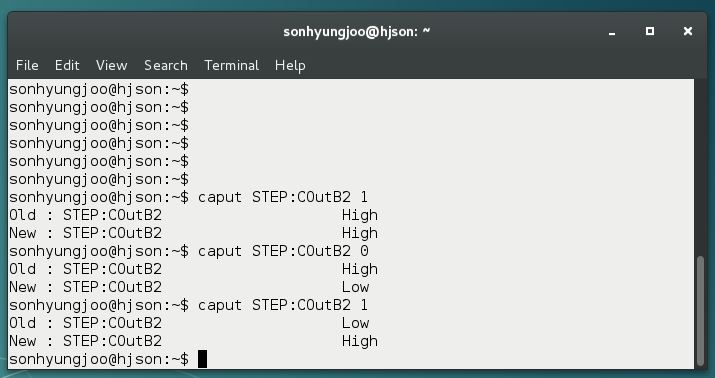
\includegraphics[width=0.9\textwidth]{./picture/caput.JPG}
	\caption{
		Address matching test on IOC
	}
	\label{fig:}
\end{figure}

\begin{figure}[h]
	\centering
	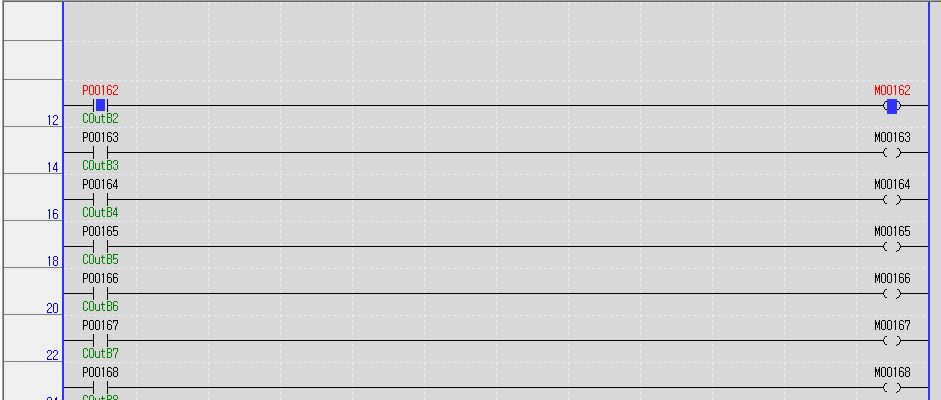
\includegraphics[width=0.9\textwidth]{./picture/ladder_output.JPG}
	\caption{
		Address matching test on PLC
	}
	\label{fig:}
\end{figure}

Figure 10에서 처럼 STEP:COutB2 라는 bit PV에 1을 넣어주면, Figure 11의 PLC bit address P00162 가 ON 되는 것을 알 수 있다. STEP:COutB3 의 Bit에 1을 넣어주면 PLC bit P00163 이 ON 될 것이다. \\

EPICS IOC의 PV와 PLC의 Memory address를 Matching 시키는 방법은 Figure 12와 같이 설정한다.

\begin{figure}[h]
	\centering
	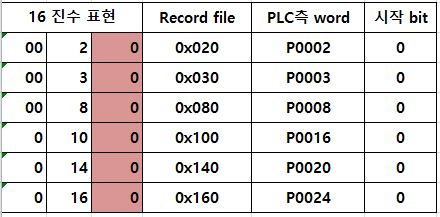
\includegraphics[width=0.9\textwidth]{./picture/MAtching.JPG}
	\caption{
		Address matching method
	}
	\label{fig:}
\end{figure}

위의 Record file에 설정해 준 0x100 은 16진수의 값으로써 PLC측의 시작 address와 일치한다. Figure 12에서 16진수 100은 PLC측 10진수 160을 말하므로 STEP:COutB0 의 값은 PLC측의 P00160 bit와 Matching 된다. 만약 0x100 대신 0x160을 넣었다면 STEP:COutB0 의 값은 PLC측의 P00240 bit와 Matching 되는 것이다. 0x000 의 형태가 아니라 0000의 형태로 값을 넣어주면 16진수가 아니라 8진수로 계산해서 PLC측의 memory와 Matching 시켜야 한다. 


\section{Summary}
현재 Step Motor Testbed의 제어부는 LS PLC로 구성되어 있다.이를 EPICS 환경에 통합시키기 위해서 EPICS Community에서 제공하는 Modbus 드라이버를 사용하여 EPICS IOC를 구성하였다. 실제 Step motor 제어에 필요한 로직은 모두 PLC에서 구성되었으며 Local UI인 M2I touch panel에서 시스템을 구동할 수 있다. LS PLC는 국산 PLC로써 다른 외산 고급 메이커인 AB PLC 및 SIMENS PLC와는 달리 소프트웨어가 무료이고 하드웨어가 저렴하며 네트워크 및 래더의 구성이 비교적 쉬운 것을 장점으로 들 수 있다. 그러나 국내외의 가속기에서 사용된 사례가 없어 그 신뢰성에 대한 데이터가 없는 것이 단점이라 할 수 있다.
  




\end{document}
